
\maketitle% this prints the handout title, author, and date

\begin{abstract}
\noindent
The objective of this lab is to determine the viscosity-average molecular weight of poly(vinyl alcohol) (PVOH) and the fraction of ``head-to-head'' monomer linkages in the polymer.\thanks{Transcribed (with corrections) from \textcite{halpern97}.} % Most of text available at https://books.google.com/books?id=Pe0J-vDm_TMC&pg=PT392
\end{abstract}

\section{Introduction} % (fold)
\label{sec:intro}

From a phenomenological point of view, we can say that the viscosity of a fluid is its resistance to flow. 
Viscosity measurements are often carried out for either of two main reasons. 
Viscosity is a quantitative property of a fluid and, although a particular sample might be highly complex, such as a blend of various resins or polymers, its viscosity serves to represent a physical property of that system. 
Viscosity, therefore, can be used as an empirical index in quality-control applications concerning, for example, oils and resins, latex paints, or chocolate mousse. 
Another motivation for measuring viscosity is to determine a fundamental and intrinsic property of a liquid (as a solvent medium): the rate of mass transport, or diffusion, within the medium. 
In this application, for example, viscosity data can provide important information about chemical reaction kinetics. 

\begin{figure}[htb]
	\centering
	\begin{tikzpicture}[scale=1.5]
		\tikzset{arrows=-Latex}
		\draw[thick,-]	(-2,0.15)	--	(4.6,0.15);
		\draw[thick,-]	(-2,2.8)	--	(4.6,2.8);
	
		\node	(A)	at	(0,2.5)	{};
			\node	(B)	at	(1,2.5)	{};
			\node	(C)	at	(2,2.0)	{};
			\node	(D)	at	(1,2.0)	{};
		\node	(E)	at	(0,1)	{};
			\node	(F)	at	(1,0.5)	{};
			\node	(G)	at	(2,0.5)	{};
			\node	(H)	at	(1,0.5)	{};
		\node(I)	at	(-0.75,1)	{};
		\node(J)	at	(-0.75,1.75)	{$\odif{z}$};
		\node(K)	at	(-0.75,2.5)	{};
		\node(L)	at	(1.5,2.6)	{$\odif{A}$};
		
		% Draw axes, arrows
		\draw[thick]	(-1.8,0.5)	--	(-1.8,1.5) node[left]{$z$}	--	(-1.8,2.5);
		\draw[thick]	(-1,0)	--	(1,0) node[below]{$x$}	--	(3,0);
		\draw	(J)	--	(I);
		\draw	(J)	--	(K);
		\draw[very thick]	(C)	--	(2.8,2.0) node[right]{$v_x + \odif{v_x}$};
		\draw[very thick]	(G)	--	(2.5,0.5) node[right]{$v_x$};
		\draw[very thick]	(3.5,1.25)	--	(4,1.25)node[above]{flow}	--	(4.5,1.25);

		% Draw liquid flow layers
		\draw[dashed]	(-1.5,2.5)	--	(A);
		\draw[dashed]	(-1.5,1)	--	(E);
		\filldraw[fill=lightgray,draw=black]	(0,2.5)	--	(1,2.5)	--	(2,2.0)	--	(1,2.0)	--cycle;
		\filldraw[fill=lightgray,draw=black]	(0,1)	--	(1,1)	--	(2,0.5)	--	(1,0.5)	--cycle;
		\draw	(1.3,2.6)	to [out=180,in=90]	(1,2.25);
	\end{tikzpicture}
	\label{fig:viscous_flow}
	\caption{In viscous flow, a sheet of fluid having cross-sectional area \( \odif{A} \) is subjected to a force that causes it to move faster by an amount \( \odif{V} \) than an equivalent, adjacent sheet separated by a distance \( \odif{z} \). 
	The planes of the sheets are normal to the flow direction.}
\end{figure}
Considered macroscopically, viscosity is a frictional force that arises from the directed motion of molecules past each other in the liquid state. 
From a microscopic viewpoint, viscosity reflects the energetics of molecular association in the liquid state because in order for a liquid to flow, a force must be applied to overcome the attractive forces between the molecules. 
These forces are appreciable; they are manifest, for example, as latent heat of vaporization and surface tension. 
The mathematical treatment of viscosity is best introduced by looking at \cref{fig:viscous_flow}.

A liquid is presumed to be flowing smoothly in the \( x \)-direction. 
Imagine that the liquid is composed of sheets of infinitesimal cross section \( \odif{A} \) that are oriented in the \( xy \)-plane, and that each sheet flows tangentially to its surface area, in the positive \( x \)-direction. 
If a given sheet is kept at a velocity \( v \), such that it exceeds the velocity of an adjacent sheet by an amount \( \odif{v} \), and the adjacent sheet is displaced by a distance \( \odif{z} \) the force required (per unit area) to maintain the motion of the given sheet, \( \odif{f_x} \), is given by
\begin{equation}
	\odv{f_x}{A} = \eta \pdv{v_x}{z}_{z} \, .
	\label{eq:layer_flow}
\end{equation}
The partial derivative, \( \pdv{v_x}/{z}_{z} \), is the tangential velocity gradient, and \( \eta \), the proportionality constant between \( f_x \) and this gradient, is now defined as the \emph{viscosity coefficient}. 
From \cref{eq:layer_flow}, it can be seen that the SI dimensions of the viscosity coefficient are \unit{\kg \per \m \per \s}. \Cref{eq:layer_flow} is called Newton's law of viscous flow. 
Fluids that behave according to \cref{eq:layer_flow} are called Newtonian fluids and are said to undergo \emph{laminar} flow. 
Cases of non-laminar, or non-Newtonian flow (at ordinary temperatures and pressures) are unusual but not uncommon (e.g., ``silly putty'').
Materials whose viscosity decreases at high shear rates (e.g., paints that ``thin out'' as they are applied with a brush but then stiffen when quiescent) are examples of non-Newtonian fluids.

With respect to this experiment, a useful application of \cref{eq:layer_flow} to the case of mass transport through a circular tube of small internal diameter was derived by French physicist Jean Léonard Marie Poiseuille in 1844:
\begin{equation}
	\odv{V}{t} = \frac{\pi r^4 \increment P}{8 \eta L} \, ,
	\label{eq:tube_flow}
\end{equation}
where \( \odv{V}/{t} \) is the volume flow rate of the liquid emerging from the tube, and \( r \) and \( L \) are, respectively, the radius and length of the tube.
The quantity \( \increment P \) is the pressure difference across the ends of the tube and is the driving force for the bulk flow. 
\Cref{eq:tube_flow} assumes that the flow rate is slow and uniform. 
The viscosity coefficient, \( \eta \), is called the poise in recognition of Poiseuille, and has cgs units.\sidenote{One poise, \unit{\poise}, is \qty{1}{\g \per \cm \per \s}, or \qty{1}{\dyne \s}.}
For convenience, the centipoise (\unit{\centi\poise}, \qty{e-2}{\poise}), was often used to report viscosity. 
In SI units, the viscosity coefficient is \unit{\kg \per\m \per\s}, or \qty{1}{\Pa \s}, and \( \qty{1e-3}{\Pa} = \qty{1}{\milli\Pa} = \qty{1}{\centi\poise} \).
For many common liquids at room temperature, viscosities are about \SIrange{0.2}{4}{\milli\Pa}. 


\subsection{Temperature Dependence of Viscosity} % (fold)
\label{sub:temperature_dependence_of_viscosity}

It is found that, over a reasonably wide temperature range, the viscosity of a pure liquid increases exponentially with the inverse absolute temperature.
This relationship was first expressed quantitatively by Swedish physicist and chemist Svante Arrhenius in 1912:\sidenote[][-2\baselineskip]{Arrhenius is more famously associated with a similar equation that expresses the temperature dependence of a rate constant.}
\begin{equation}
	\eta = A \exp\br{\frac{E_\eta}{R T}} \, ,
	\label{eq:arrhenius_visc}
\end{equation}
where \( A \) is a constant for a given liquid and \( E_\eta \) is sometimes called the activation energy to viscous flow of the liquid.
Several theories have been proposed to rationalize \cref{eq:arrhenius_visc}.
Simply viewed, however, if a molecule is to undergo transport in the bulk medium, an energy barrier must be surmounted in order for it to ``squeeze'' past its neighbors.
In so doing, the transported molecule is overcoming intermolecular attractive forces.
A plot of \( \ln{\eta} \) vs. \( 1/T \) (sometimes called an Arrhenius plot) should, according to \cref{eq:arrhenius_visc}, be linear and have a slope equal to \( E_\eta / R \).

% % subsection temperature_dependence_of_viscosity (end)

% section intro (end)

\section{The Ostwald Viscometer} % (fold)
\label{sec:the_ostwald_viscometer}

The apparatus used in this experiment is called an Ostwald viscometer, shown in \cref{fig:viscometer}. 
Its design reflects the application of Poiseuille's law in that the liquid whose viscosity is being measured flows through a uniform capillary tube. 
In principle, the viscosity of a fluid could be measured absolutely using \cref{eq:tube_flow} if its flow rate was determined and the physical dimensions of the viscometer were known. 
However, it is more practical to calibrate a given viscometer with a liquid of known viscosity. 
The wisdom of this empirical approach can be appreciated by noting that, from Poiseuille's law, the viscosity depends on \( r^4 \); thus, the error in measuring the capillary radius enters fourfold into the measured viscosity.

\begin{marginfigure}
	\centering
	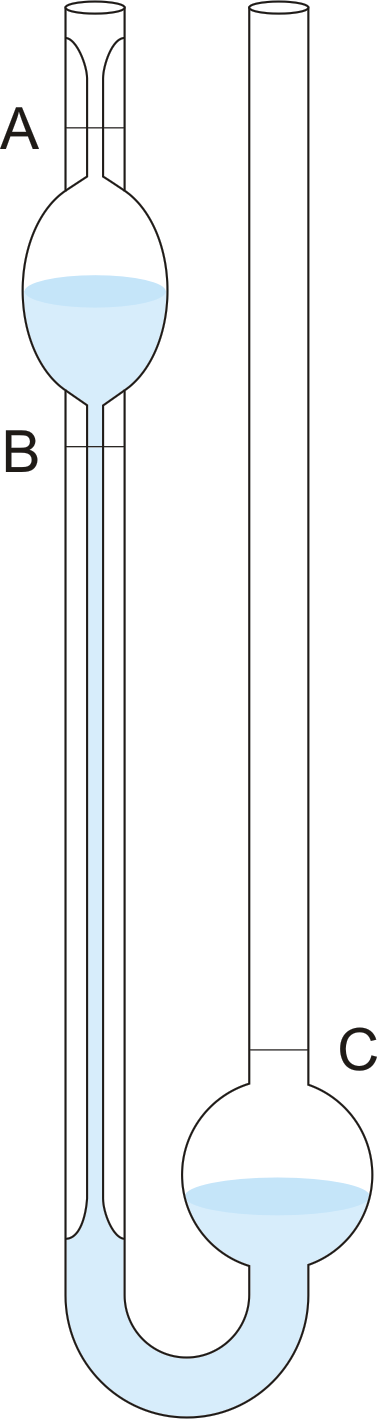
\includegraphics[width=0.6\textwidth]{images/ostwald_viscometer.png}
	\caption{Illustration of an Ostwald viscometer. 
		The left arm consists a vertical section of precise narrow bore (the capillary). 
		Above and ``below'' the bulb are a pair of large reservoirs.
		Two marks (A and B) above and below the upper bulb indicate a known volume. 
		\footnotesize{Image source: ``Ostwald’s viscometer.'' \emph{Croatian-English Chemistry Dictionary \& Glossary} 20 Oct. 2018. \url{https://glossary.periodni.com}.}}
	\label{fig:viscometer}
\end{marginfigure} 

Operationally, the experiment consists of measuring the time required for a given volume of liquid to flow through the viscometer capillary. 
The driving pressure that forces the liquid through the capillary is provided by gravity; hence, the difference in driving force between the measured and calibrating liquids is accounted for through the respective densities of these liquids. 
The Ostwald viscometer is designed to keep the separation of the upper and lower levels of the flowing liquid as constant as possible. 
This is accomplished by the spherical bulbs on the feed and receive ends of the apparatus. 
The volume of liquid that flows through the viscometer is determined by the positions of two lines (A and B in \cref{fig:viscometer}) that are inscribed on either side of the feed bulb. 
These lines are called fiducial (fixed reference) marks. 
The experiment, then, consists of measuring the time required for the liquid meniscus to pass between the upper and lower fiducial marks of the viscometer.

We can readily integrate Poiseuille's law \cref{eq:tube_flow} and then express the viscosity as
\begin{equation}
	\eta = \frac{\pi r^4 P t}{8 V L} \, ,
	\label{eq:viscometer_visc1}
\end{equation}
where \( t \) is the elapsed time and \( V \) is the volume of liquid passing through the viscometer. 
The latter is constant for a given viscometer. 
Because the hydrostatic pressure, \( P \), is proportional to the liquid density, \( \rho \) (the height is the same for both liquids), and the physical characteristics of the viscometer can be lumped into a constant, \( k_\mtext{inst} = r^4/\br{8 V} \), the expression for viscosity becomes simply
\begin{equation}
	\eta = k_\mtext{inst}\, \rho t \, .
	\label{eq:viscometer_visc2}
\end{equation}
Thus, if you measure the flow time, \( t \), for a liquid having a density \( \rho \), you can determine its viscosity relative to that of some reference liquid, i.e.,
\begin{equation}
	\eta = \frac{\eta_\mtext{ref} \, \rho t}{\rho_\mtext{ref} \, t_\mtext{ref}} \, ,
	\label{eq:ref_viscosity}
\end{equation}
where \( \eta_\mtext{ref} \), \( \rho_\mtext{ref} \), and \( t_\mtext{ref} \) are the viscosity, density, and flow time of the \emph{reference} liquid, usually water. 
It is important that you carry out the set of measurements at a known and controlled temperature; hence, the \( \eta_\mtext{ref} \) value pertains to this temperature. 
For highly precise determinations of viscosity a kinetic-energy correction term must be subtracted from \cref{eq:viscometer_visc2}. 
Because this correction is usually less than \qty{1}{\percent} of the quantity \( \br{c \rho t} \), it can be ignored.

% section the_ostwald_viscometer (end)

\section{Polymers} % (fold)
\label{sec:polymers}

One of the fundamental molecular properties used to characterize a polymer is its molecular weight. Many of the physical characteristics of polymeric materials can be associated with the shape and weight distribution of the polymer. Some experimental techniques used to obtain this information are viscosity, osmotic pressure, and light scattering measurements. These measurements are made not on the polymer itself but on solutions containing the dissolved polymer. Because the viscosity and osmotic pressure of these solutions depend systematically on the concentration of polymer, they are called \emph{colligative properties}. 

We seek a relationship between the viscosity of a solution containing a dissolved high molecular weight polymer and some molecular weight property of the polymer itself. 
A significant contribution to this field was made by \textcite{einstein06}, who showed that the \emph{fractional change} in the viscosity of a solution---relative to the pure solvent---is related to the fraction of the total volume of solution occupied by the solute, in this case the polymer. 
It is assumed that the solute has simple spherical geometry. 
Thus the relevant equation is
\begin{equation}
	\frac{\eta - \eta_0}{\eta_0} \equiv \eta_\mtext{sp} = \frac{C v_\mtext{solute}}{V} \, ,
	\label{eq:frac_visc1}
\end{equation}
where \( \eta \) and \( \eta_0 \) are the respective viscosities of the solution and the pure solvent. 
The term \( \eta_\mtext{sp} \) (which is dimensionless and positive because \( \eta > \eta_0 \)) is defined as the \emph{specific viscosity} and is proportional to the ratio of the solute volume, \( v_\mtext{solute} \), to that of the solution, \( V \). 
Thus, \( \eta_\mtext{sp} \) is a \emph{colligative property} because its value depends on the amount of polymer in solution, i.e., its concentration. 
The constant \( C \) has a theoretical value of \( 5/2 \) (for spherical solutes). 

For a solution containing \( N \) spherical solute molecules, each of radius \( R \), \cref{eq:frac_visc1} becomes (using \( C = 5/2 \) and \( v_\mtext{solute} = 4 \pi R^3 / 3 \))
\begin{equation}
	\eta_\mtext{sp} = \frac{10 \pi R^3 N}{3 V} \, .
	\label{eq:frac_visc2}
\end{equation}
\Cref{eq:frac_visc2} can more conveniently be expressed in terms of the mass concentration of the solute in the solution \( c_m \) (defined as grams per milliliter), and the \emph{molecular} mass of the solute, \( m \), as (noting that \( c_m = N_A m / V \))
\begin{equation}
	\eta_\mtext{sp} = \frac{10 \pi R^3 c_m}{3 m} \, .
	\label{eq:frac_visc3}
\end{equation}
The colligative nature of \( \eta_\mtext{sp} \) is explicit in \cref{eq:frac_visc3} because of the \( c_m \) dependence. 

Another quantity that will prove to be very useful is the \emph{intrinsic viscosity}, \( [\eta] \) (sometimes referred to as the Staudinger index):
\begin{equation}
	[\eta] \equiv \lim_{c_m \to 0}\br{\frac{\eta_\mtext{sp}}{c_m}} = \frac{10\pi R^3}{3 m} \qquad \unit{\cm\cubed \per \g}
	\label{eq:staud_ind1}
\end{equation}
The limit of infinite dilution \( \br{ c_m \to 0} \) is required to define a viscosity property that is intrinsic to the solute (in the given solvent), i.e., independent of the concentration. 
This approach essentially eliminates problems caused by the fact that the bulk properties of the polymer solution vary with concentration. 

The limiting condition defined in \cref{eq:staud_ind1} is needed to define \( [\eta] \) because the reduced specific viscosity (i.e., \( \eta_\mtext{sp}/c_m \)) depends on the polymer concentration due to shear forces between the dissolved macromolecule and the solvent medium. 
This concentration dependence is observed to follow the relation
\begin{equation}
	\frac{\eta_\mtext{sp}}{c_m} = [\eta] + k_\mtext{Hug} [\eta]^2 c_m + k' c_m^2 \, ,
	\label{eq:conc_dep}
\end{equation}
where \( k_\mtext{Hug} \), known as the Huggins constant, has a value of about \num{2} for rigid, uncharged spheres, and about \num{0.35} for flexible polymers in a ``good'' solvent.\autocite{tanford61} 
The higher-order term in \( c_m \) in \cref{eq:conc_dep} can often be neglected. 
From \cref{eq:frac_visc3} we can see that the ratio \( \eta_\mtext{sp}/c_m \) is not a colligative quantity; it is equal to an intrinsic property of the solute itself, namely, \( 10 \pi R^3 / 3 m \). 
The intrinsic viscosity has dimensions of \unit{\cm\cubed \per\g} and is perhaps analogous to a molar volume. 
Because both \( \eta_\mtext{sp} \) and \( c_m \) are experimental quantities, \cref{eq:conc_dep} can be used to obtain \( [\eta] \) by extrapolation to zero concentration.

It is interesting to note that, if \( R \) is known, \cref{eq:staud_ind1} can be used to determine \( m \), the molecular mass of the solute, from \( [\eta] \). 
Furthermore, the molecular weight of the solute divided by its mass provides Avogadro's number, \( N_A \), which suggests an experimental approach for obtaining this fundamental constant. 
Conversely, if \( m \) is known, a value of the solute radius, \( R \), can be determined from \( [\eta] \). 
Following this reasoning, Einstein was able to obtain a satisfactory value of Avogadro's number as well as the molecular radii of carbohydrates. 
Few other direct experimental methods can be used to measure Avogadro's number.

Intrinsic viscosity measurements can be applied to a high molecular weight polymer to obtain its (spherical) radius or its molecular weight. 
Remember that the value of \( R \) in \cref{eq:frac_visc2,eq:frac_visc3,eq:staud_ind1} denotes the \emph{effective} radius of the solute, because the solute may not be exactly spherical, and in addition, the solute may be associated with a (possibly large) number of solvent molecules. 
This effective radius is referred to as the \emph{hydrodynamic radius} and can, in principle, vary for a given solute from solvent to solvent depending on what shape the solute adopts in a particular solvent, that is, the extent to which solvent molecules penetrate or stick to the solute.

Another complication that can be anticipated in applying \cref{eq:staud_ind1} to molecules is that the assumption of spherical geometry may be invalid in some cases. 
Deviations from spherical geometry would manifest themselves theoretically in that \( C \) (in \cref{eq:frac_visc1}) would have values other than \num[parse-numbers=false]{5/2}. 
In principle, this can be accounted for if the correct \emph{solvated} molecular shape (oblate or prolate spheroid, oblong, etc.) is known.

A more serious problem encountered in dealing with high polymers is the fact that these systems consist of polymers of various chain lengths. 
Thus these are not homogeneous solutes (monodisperse) but have a distribution of molecular weights and are called \emph{polydisperse}. 
The degree to which a polymer is polydisperse depends on the conditions under which it is synthesized. 
Although in theory a polydisperse polymer can be fractionated into groups that have a more narrow molecular weight distribution (nearly monodisperse), this is often a long and tedious process. 
Measurements on raw, polydisperse polymer solutions provide information that is averaged over the molecular weights (and sizes) of the polymer. 
Such is the case in viscosity measurements.

\begin{marginfigure}
	\begin{tikzpicture}
	  \def\InnerRadius{0.2cm}
	  \def\OuterRadius{1.5cm}
	  \def\PointsPerCircle{20}
	  \def\NumOfCircles{3}
	  \def\DeltaAngle{15}
	  \pgfmathsetseed{104}
	  \draw[]
	     plot[
	       smooth cycle,
	       samples=\PointsPerCircle*\NumOfCircles + 1,
	       domain=0:360*\NumOfCircles,
	       variable=\t,
				 tension=6
	    ]
	      ( \t + rand*\DeltaAngle:
	        {random*(\InnerRadius) + random*(\OuterRadius-\InnerRadius)})
	  ;
	\end{tikzpicture}
	\caption{Schematic diagram of a linear chain polymer in a random-coil configuration.}
	\label{fig:poly_ball}
\end{marginfigure}
In order to apply \cref{eq:staud_ind1} to a system that is composed of a high molecular weight polydisperse polymer, a statistically averaged form of the molecular ``radius'' has to be used. 
In this experiment, the polymer studied---like many others---is a \emph{linear} chain system, which means that the macromolecule is formed from a large number of monomer units in such a way that monomers add to the developing polymer chain without branching. 
Although the molecule is called a ``linear'' chain, its geometry surely does not resemble a straight-line assembly of monomer units. 
Rather, it is coiled up and adopts an overall shape that is approximately spherical. It may be thought to resemble a loosely tangled ball of yarn, illustrated in \cref{fig:poly_ball}.
This so-called random coil is not a static structure but continually undergoes contortional motion as the different segments go through various conformational transitions. 
On a time-averaged basis, however, we can define a statistical radius called the \emph{radius of gyration}, \( R_g \). 
This characteristic property is expressed quantitatively as
\begin{equation}
	R_g = \sqrt{\frac{I}{m}} \, ,
	\label{eq:rad_gyr}
\end{equation}
where \( m \) is the molecular mass and \( I \) is the moment of inertia, a second-order moment defined as
\begin{equation}
	I = \sum_i m_i r_i^2 \, ,
	\label{eq:mom_inert}
\end{equation}
in which the sum over all the point masses, \( m_i \) (atoms), of the molecule, and \( r_i \) is the distance to the \( i\mtext{th} \) atom from the center of mass. 
We can calculate \( I \) only if we adopt some (static) structural model of the polymer. 
If we substitute the radius of gyration for the unique-valued radius \( R \) in \cref{eq:staud_ind1}, we have
\begin{equation}
	[\eta] = \frac{N_A 10 \pi R_g^3}{3 M} \qquad \unit{\cm\cubed \per \g} \, ,
	\label{eq:staud_ind2}
\end{equation}
where \( M \), the molecular weight (along with \( N_A \)) replaces the molecular mass, \( m \).

If we now assume that the linear chain polymer is constructed of \( N \) monomer units linked together in such a way that \emph{each} link is rotationally flexible, or unhindered (freely jointed chain), it can be demonstrated that the radius of gyration is proportional to the square root of the number of links in the polymer chain; thus \( R_g \propto \sqrt{N} \). 
This important conclusion is developed through the application of statistical mechanics to polymers.\autocite{halpern97} Thus
\begin{equation}
	[\eta] = K' \sqrt{M} \, ,
	\label{eq:staud_ind3}
\end{equation}
where \( K' \) is a proportionality constant that contains the conversion factor between \( R_g \) and \( \sqrt{M} \). 
\Cref{eq:staud_ind3} is of particular importance in this experiment. 
It relates a measurable quantity, the intrinsic viscosity, to the desired molecular weight of the polymer. Although the square root dependence of \( [\eta] \) on molecular weight is actually observed for some monodisperse polymer solutions, many others deviate from \cref{eq:staud_ind3}. 
The reasons for these discrepancies have to do with the nature of solvation and the effects brought about by solvent association on the structure of the polymer solute. 
Thus, the molecules of a ``good'' solvent enter into the polymer coils to maximize solvolytic associations, and the polymer expands. 
Looked at another way, the polymer ``swells'' our into the solvent. 
In a ``poor'' solvent, on the other hand, the polymer knots up into itself and avoids the interactions with the solvent molecules. 
As you might expect, the solubility of a given polymer is larger in a good solvent than in a poor one, as illustrated in \cref{fig:poly_solv}. 

\begin{marginfigure}
	\centering
	\subfloat[][good solvent]{%
		\begin{tikzpicture}
			\def\InnerRadius{0.2cm}
			\def\OuterRadius{1.5cm}
			\def\PointsPerCircle{20}
			\def\NumOfCircles{3}
			\def\DeltaAngle{5}
			\pgfmathsetseed{83}
				\draw[]
					plot[
						smooth cycle,
						samples=\PointsPerCircle*\NumOfCircles + 1,
						domain=0:360*\NumOfCircles,
						variable=\t,
						 tension=4
					]
						( \t + rand*\DeltaAngle:
							{random*(\InnerRadius) + random*(\OuterRadius-\InnerRadius)})
						;
		\end{tikzpicture}%
        \label{fig:poly_solv_good}%
    }\\%
	\subfloat[][poor solvent]{%
		\begin{tikzpicture}
			\def\InnerRadius{-0.1cm}
			\def\OuterRadius{0.7cm}
			\def\PointsPerCircle{20}
			\def\NumOfCircles{3}
			\def\DeltaAngle{5}
			\pgfmathsetseed{83}
				\draw[]
					plot[
						smooth cycle,
						samples=\PointsPerCircle*\NumOfCircles + 1,
						domain=0:360*\NumOfCircles,
						variable=\t,
						tension=2
					]
						( \t + rand*\DeltaAngle:
							{random*(\InnerRadius) + random*(\OuterRadius-\InnerRadius)})
						;
		\end{tikzpicture}%
        \label{fig:poly_solv_poor}%
    }%
	\caption{Schematic diagram of a random-coil polymer in a ``good'' solvent (\cref{fig:poly_solv_good}) and a ``poor'' solvent (\cref{fig:poly_solv_poor}).}
	\label{fig:poly_solv}
\end{marginfigure}

Another important consideration we have ignored thus far in the discussion is called the ``excluded volume.''
This is the effective space that is inaccessible to a random coil or freely jointed chain. 
This volume cannot be occupied because the segments of the polymer avoid each other as they become too close during the twisting and turning that the polymer undergoes. 

A more general relationship between the intrinsic viscosity and molecular weight is provided by the Mark-Houwink equation:
\begin{equation}
	[\eta] = K M^a \qquad \unit{\cm\cubed \per \g} \, ,
	\label{eq:mark_houwink}
\end{equation}
where \( K \) and \( a \) are parameters that depend on the particular polymer, the solvent medium, and the temperature. 
Typically, \( a \) ranges from \numrange{0.5}{0.8}.\sidenote{See \cref{eq:staud_ind3}} 
The Mark-Houwink parameters are obtained from log-log plots of \( [\eta] \) vs. \( M \) for a series of monodisperse polymers. 
Agreement between \( K \) and \( a \) values obtained by different workers is often apparently poor.\autocite{immergut75} 
For example, for PVOH in water at \qty{25}{\celsius}, the following parameters showing in \cref{tab:pvoh_mh_param} have been reported. 
\begin{table}[hb]
	\centering
	\sisetup{table-number-alignment = center}
		\begin{tabular}{SSSr}%
			\toprule
			{\( K \)}	&	{\( a \)}	&	{Molecular Weight Range}	&	Source	\\
			{(\unit{\cm\cubed\per\g})}	&		&	{(\unit{\kilo\dalton})}	&			\\
			\midrule
			0.020			&	0.76	&	\numrange{6}{210}	&	{\autocite{flory48,flory50}}	\\
			0.30			&	0.50	&	\numrange{9}{170}	&	{\autocite{dialer52}}				\\
			0.14			&	0.6		&	\numrange{10}{70}	&	{\autocite{dieu54}}					\\
			\bottomrule
		\end{tabular}
	\caption{Mark-Houwink parameters for PVOH in water at \qty{25}{\celsius}.}
	\label{tab:pvoh_mh_param}
\end{table}


We can obtain the molecular weight in explicit form from \cref{eq:mark_houwink}:
\begin{equation}
	M_v = \br{\frac{[\eta]}{K}}^{1/a} \, .
	\label{eq:vol_avg_weight}
\end{equation}
This expression (in which \( [\eta] \) has dimensions of \unit{\cm\cubed \per \g}) is the computational basis of the experiment; it can be applied to \emph{poly}disperse PVOH (which is used in this experiment), but the molecular weight obtained from \cref{eq:vol_avg_weight} is a \emph{viscosity-average} molecular weight, \( M_v \). 
Statistically, this quantity is different from the \emph{number-average} molecular weight, \( M_n \), which is obtained, for example, from osmotic pressure measurements. 
\( M_n \) is defined as 
\begin{equation}
	M_n = \sum_i f_i M_i \, ,
	\label{eq:num_avg_weight}
\end{equation}
where \( f_i \) is the fraction of polymers having molecular weight \( M_i \); the sum in \cref{eq:num_avg_weight} extends (in theory) from \num{0} to \( \infty \). 

\textcite{schaefgen48} have shown that the relationship between \( M_v \) and \( M_n \) is
\begin{equation}
	\frac{M_v}{M_n} = \br{\br{1 + a} \cdot \GammaFunc\br{1 + a}}^{1/a} \, ,
	\label{eq:mol_weight_ratio}
\end{equation}
where \( a \) is the same parameter used in \cref{eq:mark_houwink} and \( \GammaFunc\br{x} \) denotes the \emph{gamma function}, whose value (for a given \( x \)) can be obtained from mathematical tables. 
For example, for \( a = 0.76 \) (for PVOH in water at \qty{25}{\celsius}),\autocite{flory48} the ratio in \cref{eq:mol_weight_ratio} is 
\begin{equation}
	\frac{M_v}{M_n} \equiv S = 1.89 \, .
	\label{eq:mol_weight_ratio_ex}
\end{equation}
For \( a = 0.50 \) and \num{0.60},\sidenote{See \cref{tab:pvoh_mh_param}} \( S \) is \num{1.77} and \num{1.81}, respectively. 

% section polymers (end)

\section{Chemical Bonding in PVOH} % (fold)
\label{sec:chemical_bonding_in_pvoh}

Poly(vinyl alcohol) is obtained from the hydrolysis of poly(vinyl acetate). 
The latter is synthesized from vinyl acetate monomers. 
Let us consider the question of how the vinyl acetate monomers link up to form the poly(vinyl acetate) polymer. 
The structure of vinyl acetate is shown in \cref{fig:vinyl_acetate}.
\begin{marginfigure}
	\centering
	\chemfig{[:60]C(-[:-120]H)(-[:120]H)=[0]C(-[:-60]H)-O-[0]C(-[:-60]CH_3)=O}
	\caption{Vinyl acetate monomer}
	\label{fig:vinyl_acetate}
\end{marginfigure}
It is an unsymmetrically substituted ethylene molecule, since only one end of the molecule is derivatized. 
Thus, when a monomer is about to bond to the ``growing'' end of a polymer chain, it can do so in two ways with respect to the previously bonded monomer unit: either the carbon atom containing the functional group, \ch{X} (\ch{C$\sb{a}$}), can bond to the terminal end of the polymer chain, or the unfunctionalized carbon (\ch{C$\sb{b}$}) can form the bond. 
These alternatives are illustrated in \cref{fig:growth_directions}. 
An attachment in which the functional groups alternate is called ``head-to-tail'', while the one in which they are attached on adjacent carbon atoms is referred to as a ``head-to-head'' linkage. 
Because a head-to-head linkage involves considerable steric repulsion between the functional groups (ethyl will have been added to \emph{adjacent} carbon atoms on the polymer chain to form \iupac{1,2-substituents}), it proceeds more slowly than a head-to-tail linkage. 
Therefore, a polymer will have a predominance of the latter arrangements, and the functional groups will, for the most part, alternate in their positions on the polymer backbone (i.e., repetitive \iupac{1,3-substituents}). 
\begin{figure}[htb]
	\captionsetup[subfigure]{farskip=20pt,captionskip=20pt}
	\subfloat[][head-to-head growth]{%
		\chemfig{
			CH-CH(-[2]R)-[@{op, 0.5}]CH-CH(-[2]R)-[@{cl,0.5}]CH-CH(-[2]R)-{\color{blue}C_\emph{a}}(-[2]R)={\color{red}C_\emph{b}}(-[2]H)-H}
		\makepolymerdelims{35pt}[7pt]{op}{cl}
		\label{fig:h2h_growth}
	} \\
	\subfloat[][head-to-tail growth]{%
		\chemfig{
			CH-CH(-[2]R)-[@{op, 0.5}]CH-CH(-[2]R)-[@{cl,0.5}]CH-CH(-[2]R)-{\color{red}C_\emph{b}}(-[2]H)={\color{blue}C_\emph{a}}(-[2]R)-CH_3}
		\makepolymerdelims{35pt}[7pt]{op}{cl}
		\label{fig:h2t_growth}
	}
	\caption{Comparison of head-to-head growth (\cref{fig:h2h_growth}) and head-to-tail growth (\cref{fig:h2t_growth}).}
	\label{fig:growth_directions}
\end{figure}

Note also that if, after a head-to-head linkage has taken place, the next monomer attaches in a tail-to-tail fashion, the resulting arrangement between the substituents is a \iupac{1,4-disubstituted} configuration. 
Considering the way this experiment is to be carried out,\sidenote{See the procedure} only the presence of head-to-head attachment is chemically significant. 
These result in the formation of \iupac{1,2-disubstituted} structures on the polymer chain. The number of such events that occur in polymerization relative to the more common head-to-tail attachment (and thus \iupac{1,3-disubstituted} structures) is of interest because the physical and chemical properties of the polymer depend on the fraction of such head-to-head linkages. 
Thus, some analytical method for establishing this information is desirable. 

In the case of the polymerization of vinyl acetate and the subsequent hydrolysis of the polymer to form PVOH, the consequence of the head-to-head linkage is the formation of a \iupac{1,2-diol} (or \emph{vicinal glycol}). 
The more common head-to-tail linkages result in the formation of \iupac{1,3-diols}. 
The presence of \iupac{1,2-diol} structures in the polymer can be conveniently distinguished from the \iupac{1,3-diols} by a chemical means. 
The \iupac{1,2-diol} is specifically cleaved (and oxidized) using periodic acid, \ch{HIO4}. 
Actually, the reagent used is the periodate anion (from \ch{KIO4}), which hydrolyzed in water to form \ch{HIO4}.
The reaction is shown in \cref{fig:diol_cleavage}. 
Hence, treatment of a PVOH sample with \ch{KIO4} will split the polymer wherever a \iupac{1,2-diol} structure exists. 
This results in a decreases in the (average) molecular weight of the polymer, and this change can be detected via viscosity measurements. 
\setchemfig{atom style={scale=0.80}}
\begin{figure}[htb]
	\subfloat{
		\schemestart
			\chemfig{[:-30]--[:30](-[2]OH)--[:30](-[2]OH)-} \arrow{->[\ch{HIO4}]} \quad \Large{N.R.}
		\schemestop} \\
	\subfloat{
		\schemestart
			\chemfig{[:-30]--[:30](-[2]OH)-(-[6]OH)-[:30]-} \arrow{->[\ch{HIO4}]}
				\chemfig{[:-30]--[:30](=[2]O)-H} \arrow{0}[,0] \+ \arrow{0}[,0] \chemfig{[:-30]O=[:90](-[:150]H)-[:30]-}
		\schemestop
		}
	\caption{Mechanism for cleavage of a vicinal diol.}
	\label{fig:diol_cleavage}
\end{figure}

If we assume that the cleavage reaction is \qty{100}{\percent} effective (so that all the \iupac{1,2-diol} linkages are cleaved), the increase in the number of solute molecules in the solution after treatment with \ch{KIO4} divided by the total number of monomer units represented in the polymer sample is equal to the ratio of \iupac{1,2-diol} structures to the total \iupac{1,2-diol} \emph{and} \iupac{1,3-diol} arrangements in the system. 
This ratio, which is defined here as \( f \), can be expressed as
\begin{equation}
	f = \frac{\frac{1}{M_n'} - \frac{1}{M_n^0}}{\frac{1}{M^0}} \, ,
	\label{eq:frac_glycol}
\end{equation}
where \( M_n^0 \) and \( M_n' \) are the number-average molecular weights of the polymer in the sample before
and after the \ch{KIO4} cleavage respectively. 
\( M^0 \) is the molecular weight of the monomer unit (\ch{CH2CHOH}), which is \qty{44}{\dalton}. 
Using the relationship between the number average and viscosity-average molecular weight for PVOH,\sidenote{See \cref{eq:mol_weight_ratio_ex}} we get the following expression for the head-to-head fraction:
\begin{equation}
	f = S M^0 \br{\frac{1}{M_v'} - \frac{1}{M_v^0}}\, .
	\label{eq:h2h_frac}
\end{equation}
This equation provides the final result used in this experiment. 
It permits \( f \) to be determined from \( [\eta] \) measurements of the PVOH sample before and after cleavage by \ch{KIO4}. The value of \( S \) depends on the choice of \( a \) used in \cref{eq:mol_weight_ratio}.\sidenote{See \cref{tab:pvoh_mh_param}}

% section chemical_bonding_in_pvoh (end)


\pagebreak

\section{Safety Precautions} %(fold)
\label{sec:safety}

\begin{itemize}
	\item \ch{KIO4} is an oxidant and should be handled cautiously. 
	\item Always wear safety glasses in the laboratory.
	\item Make sure you have been shown how to use proper pipetting techniques. 
	Never pipet by mouth.
	\item Handle the viscometer carefully to avoid breakage. 
\end{itemize}
% section safety (end)


\section{Procedure} % (fold)
\label{sec:procedure}

You will be provided with a clean viscometer. 
If the viscometer appears to be dirty, do not proceed with the experiment. 
Either obtain a clean one, or take the time to clean your viscometer thoroughly. 
Consult your instructor. 
If you do not remember how to use the viscometer, review the material in Experiment 16, or ask your instructor for this information. 
A stock solution of PVOH in water (\( c_m \approx \qty{0.016}{\g \per \mL} \)) should be available; if it is not, you will be told how to prepare this solution. 
This PVOH must have been appropriately filtered before use; undissolved particles will clog the viscometer. 
You will measure the viscosities of PVOH solutions of three or four different concentrations for both the cleaved and uncleaved polymers. 
You will calibrate the viscometer using pure water. 
Temperature control for each of these measurements is important.

\subsection{Required Equipment} % (fold)
\label{sub:required_equipment}

\begin{itemize}
	\item (2) \qty{100}{\mL} volumetric flask
	\item (6) \qty{50}{\mL} volumetric flasks
	\item (1) \qty{50}{\mL} volumetric pipet
	\item (1) \qty{50}{\mL} graduated cylinder
	\item (1) pipet filler
	\item (1) Ostwald viscometer
	\item (1) temperature-controlled water bath
\end{itemize}

% subsection required_equipment (end)

\begin{enumerate}
	\item Prepare \qty{100}{\mL} of a \qty{50}{\percent} solution of the PVOH stock solution. 
	You will use this to prepare the diluted samples of the uncleaved polymer for measurement. 
	Use purified (DI, RO, or distilled) water for the dilution in the volumetric flask. 
	Cap and invert it several times gently. 
	Do not agitate, as this causes foaming. 
	Because the polymer tends to adhere to the surface of glassware, rinse the pipet with water, then acetone, immediately after use. 
	Aspirate dry. 
	Follow this procedure whenever using glassware with PVOH solutions.
	\item To prepare the cleaved polymer, pipet \qty{50}{\mL} of the stock solution into a 100-mL volumetric flask. 
	Add \qty{0.25}{\g} of \ch{KIO4} and about \qty{20}{\mL} of deionized water. 
	Cap and swirl the liquid a few times. 
	Place the mixture in a hot-water bath (\qty{\sim70}{\celsius}) for several minutes until the solid dissolves; periodically mix the solution if necessary. 
	After the solid has dissolved, remove the flask and let it cool to room temperature, then fill to the mark with deionized water. 
	Gently invert it several times. Label the flask.
	\item There are now two PVOH solutions (one cleaved and one uncleaved), each with \( c_m \) of about \qty{0.0080}{\g \per \mL}. 
	From each of these, prepare \qty{50}{\mL} of solutions corresponding to \SIlist{80;60;40}{\percent} of that concentration. 
	Make up the \qty{40}{\percent} solution from the \qty{80}{\percent} solution. 
	Label these new samples immediately after preparation. 
	Place them all in a \qty{25}{\celsius} bath.
	\item Calibrate the viscometer with purified water. 
	Pipet \qty{5}{\mL} of water into the viscometer, which is clamped and held in a \qty{25}{\celsius} bath. 
	Using a pipet bulb, carefully ``push'' the water up through the capillary tube until it is above the upper fiducial mark. 
	Remove the bulb and allow the water to drain. 
	Start the timer or stopwatch exactly as the water meniscus passes the upper fiducial mark; stop the timer just as the meniscus passes the lower mark. 
	Record this time. Repeat this measurement at three to five times. 
	Use the pipet bulb to ``reset'' the liquid. 
	Alternatively, use a flexible tube connected to an aspirator. 
	The timings should be within \qtyrange{0.2}{0.5}{\s}. 
	After the calibration is complete, remove the viscometer from the bath.
	\item Following the same procedure, measure the viscosities of the cleaved and uncleaved samples, starting with the most dilute samples. 
	Make each measurement three to five times.
\end{enumerate}

% section procedure (end)

\section{Data Analysis} % (fold)
\label{sec:data_analysis}

\begin{enumerate}
	\item Calibrate the viscometer. 
	Determine the constant \( k_\mtext{inst} \) in \cref{eq:viscometer_visc2} from the mean flow time of water and its density and viscosity at \qty{25}{\celsius}.
	\item Determine and tabulate the viscosities and specific viscosities of the PVOH samples. 
	Assume they have densities equal to that of pure water. 
	In the same table list the bulk \( c_m \) values (\unit{\g \per \mL}) of the PVOH samples.
	\item For each sample determine \( [\eta] \) for the uncleaved and cleaved polymer. 
	Also determine the Huggins constant.\sidenote{See \cref{eq:conc_dep}}
	\item Choose a set of \( K \) and \( a \) values, and using the appropriate relations, determine values of \( M_v \) for the uncleaved and cleaved PVOH, as well as the head-to-head ratio, \( f \). 
	Comment on the magnitudes of your results.
	\item Determine \( M_v \), and \( f \) for another set of \( K \) and \( a \) values and compare them with the results in step 4.
\end{enumerate}
% section data_analysis (end)

\section{Questions and Further Thoughts} % (fold)
\label{sec:questions_and_further_thoughts}

\begin{enumerate}
	\item Consult a table of mathematical functions,\sidenote{
		These can be physical tables or values coded into a software library like SciPy. SciPy documentation on the function can be found at \href{https://docs.scipy.org/doc/scipy/reference/generated/scipy.special.gamma.html}{\Verb{scipy.special.gamma}}. You should look through the help page to see how the gamma function is defined (it's closely related to factorials) and look at the examples at the bottom of the page to see how it's used.
	} and using the appropriate gamma functions and \cref{eq:mol_weight_ratio}, verify the values of \( S \) cited within and following \cref{eq:mol_weight_ratio_ex}.
	\item Using the definition of \( f \),\sidenote{See the discussion before \cref{eq:frac_glycol}} derive \cref{eq:frac_glycol} and use the result in \cref{eq:mol_weight_ratio_ex} to obtain \cref{eq:h2h_frac}.
	\item Viscosity measurements are often performed on proteins and other biopolymers. 
	What experiments could be carried out on such molecules to examine the effect of solution conditions (e.g., ionic strength, or \ch{\pH}) on the extent of denaturation (breakdown of the biologically active structure)?
	\item Specific and intrinsic viscosities provide structural information about macromolecules under the assumption that the solute is spherical.\sidenote{See \cref{eq:frac_visc1}} 
	Is this a good assumption for a polymer such as PVOH? 
	For what sort of macromolecule would you expect this assumption to be poor?
	\item How would the structure of a polymer such as PVOH in the vapor phase differ from that in aqueous solution?
	\item The intrinsic viscosity of a sample of polydisperse PVOH in water was determined to be \qty{86}{\cm\cubed \per \g} at \qty{298}{\K}. 
	Using the information in \cref{tab:pvoh_mh_param} and \cref{eq:mark_houwink}, the Mark-Houwink equation, what range of molecular weights can be reported for the polymer?
\end{enumerate}
% section questions_and_further_thoughts (end)

\section{Lab Report Guidelines} % (fold)
\label{sec:lab_report_guidelines}

Your lab report should consist of the following parts:
\begin{description}
	\item[Title, Author and Date]
	\item[Experimental Procedure] This should be a very brief general outline of the procedure, written out as a paragraph or two. Give the make and model for any major instruments you used, as well as any important settings. Note the values written on your viscometer and how time was tracked. 
	\item[Results and Discussion] This should include answers to the questions in the section ``Questions and Further Thoughts''. This should not be a separate section, but should instead be included organically in the discussion as a way of filling it out. You should include any experimental uncertainties and report the uncertainty in your final values. Calculations of uncertainties (including propagation of error) should be included in your supporting materials. 
	\item[References]
	\item[Appendix] At the very end of your report, include examples of any calculations that you did. If you performed any derivations by hand, you may attach a picture of the work, but you should try to perform all your work digitally. 
	Make sure any data analysis done with Python is clearly annotated so the reader understands what steps you took. 
\end{description}
% section lab_report_guidelines (end)
